\section{根轨迹法}

\begin{figure}[!ht]
    \centering
    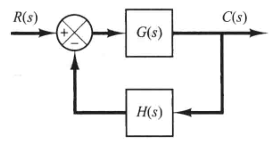
\includegraphics[width=8cm]{figures/20.png}
    \caption{闭环系统}
    \label{20}
\end{figure}

考虑如图\ref{20}所示的闭环控制系统,其传递函数为

\begin{equation*}
    \frac{C(s)}{R(s)}=\frac{G(s)}{1+G(s) H(s)}
\end{equation*}

令等式右端分母为$0$,得到特征方程:

\begin{equation*}
    1+G(s) H(s)=0
\end{equation*}

由于在$G(s)$或$H(s)$中往往存在增益$K$,可以进一步把特征方程改写为

\begin{equation*}
    1+\frac{K\left(s+z_{1}\right)\left(s+z_{2}\right) \cdots\left(s+z_{m}\right)}{\left(s+p_{1}\right)\left(s+p_{2}\right) \cdots\left(s+p_{n}\right)}=0
\end{equation*}

所谓根轨迹图,即为增益参数$K$由0变到无穷大时,闭环极点的轨迹。

典型步骤:

\begin{enumerate}
    \item 确定实轴上的根轨迹
    
    首先画出所有的开环极点与开环零点,随后根据辐角条件,确定实轴上的根轨迹。

    \item 确定渐近线
    
    \begin{align*}
        \sigma&=\frac{\sum\mbox{poles}-\sum\mbox{zeros}}{n-m}\\
        \eta_k&=\frac{(2k+1)\pi}{n-m}\quad k=0,1,2,\cdots ,n-m
    \end{align*}

    得到的$\sigma$即为渐近线与实轴的交点,$\eta_k$则是渐近线可以取到的角度。

    \item 确定分离点与会合点
    
    首先将特征方程$1+G(s) H(s)=0$化为$K=K(s)$的形式,即

    \begin{equation*}
        K=-\frac{\left(s+p_{1}\right)\left(s+p_{2}\right) \cdots\left(s+p_{n}\right)}{\left(s+z_{1}\right)\left(s+z_{2}\right) \cdots\left(s+z_{m}\right)}
    \end{equation*}

    随后令$dK/ds=0$,对应得到的$s$取值即为实轴上分离点或会合点的位置。把这个$s$代回$K=K(s)$,就可以得到该点对应的增益参数$K$。另一个方法是将式子化为关于$s$的多项式方程$f(s)=0$,由于在分离点或会合点,相当于这个方程在此处取到重根,则可以联立$df/ds=0$与$f(s)=0$,解出对应的$K$和$s$。

    \item 确定根轨迹与虚轴的交点
    
    由于极点位于虚轴上时,系统处于临界稳定状态,可以通过劳斯稳定判据确定此时对应的$K$值。使劳斯阵列第一列上的项等于零,就能得到该状态对应的$K$,再通过辅助方程,求解根轨迹与虚轴的交点。

    \item 确定极点出射角与零点入射角
    
    将试验点取在非常靠近零点/极点的地方,利用辐角条件,即可得到对应的出射/入射角度。根轨迹从极点出发,结束于零点或无穷远点处。

\end{enumerate}

MatLab中,可以直接利用\textit{rlocus}函数来绘制根轨迹图。

\begin{lstlisting}
    rlocus(num,den)
\end{lstlisting}

如图\ref{21},是一个绘制根轨迹图的例子,特征方程为:

\begin{equation*}
    0.1s^3+1.15s^2+2.5s+K(0.1s+1)=0
\end{equation*}

\begin{figure}[!ht]
    \centering
    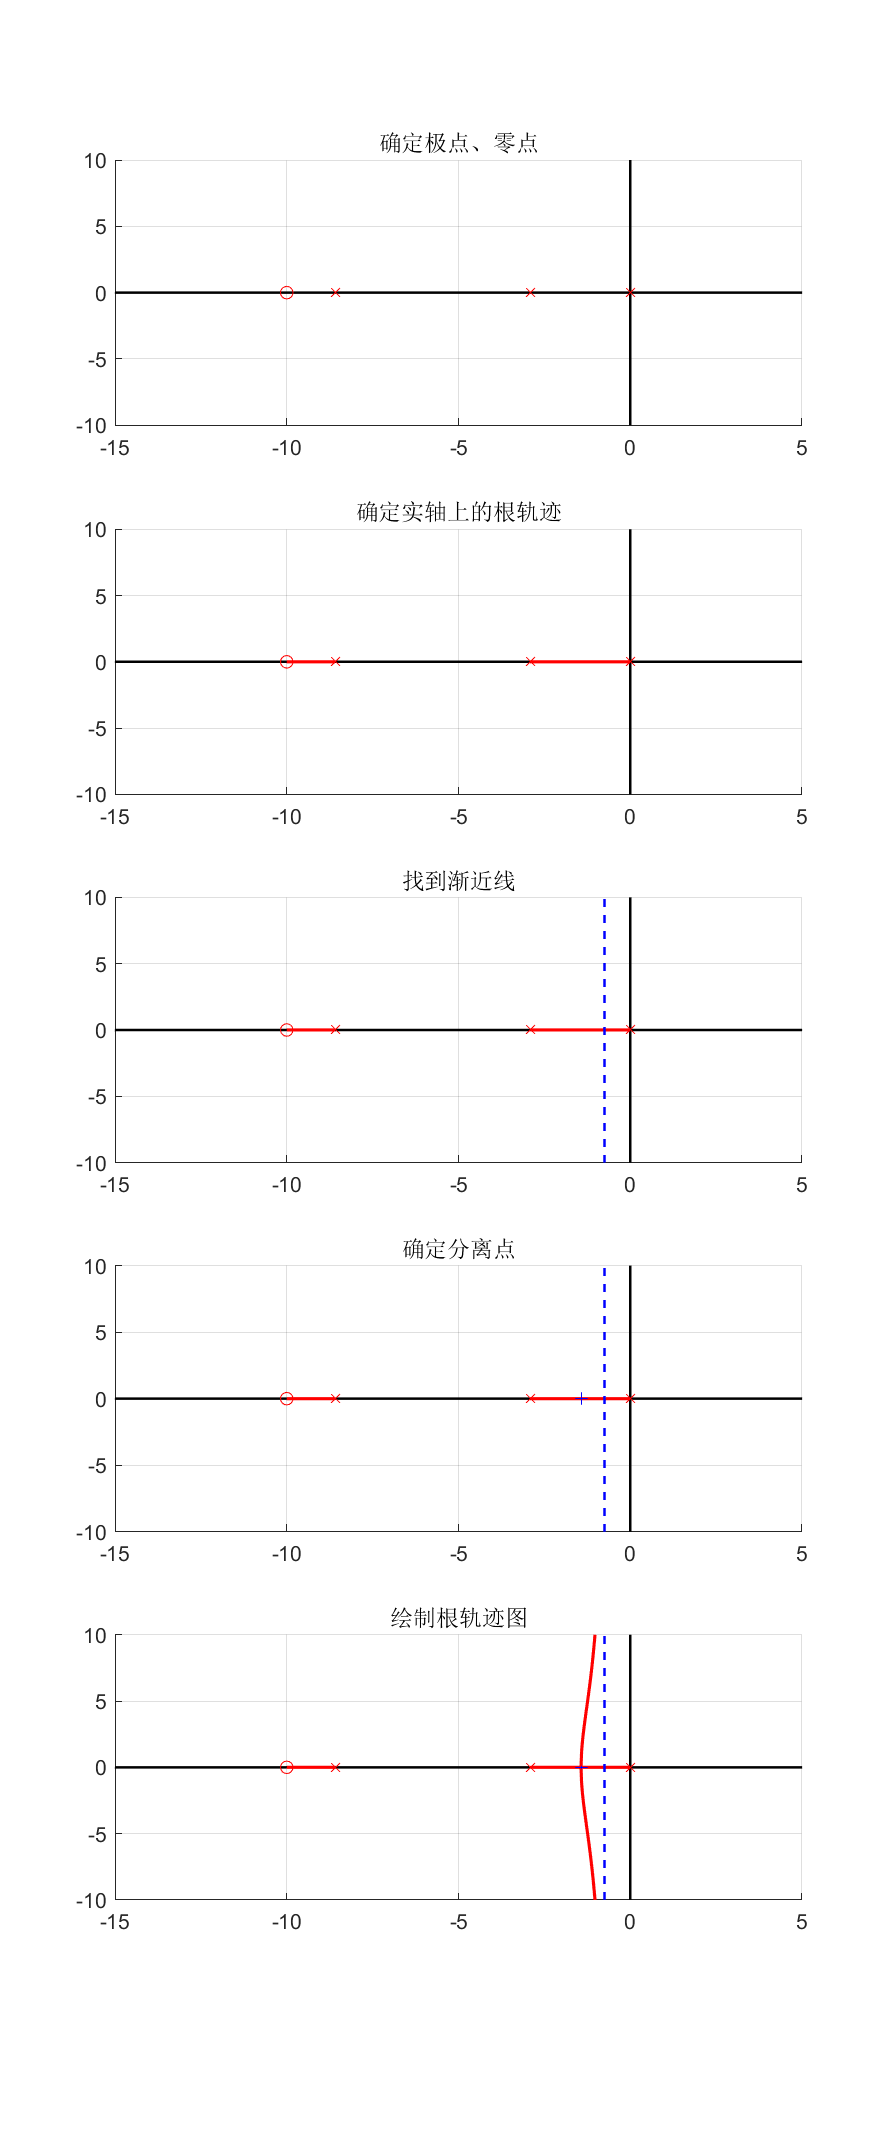
\includegraphics[width=0.5\linewidth]{figures/21.png}
    \caption{绘制根轨迹图}
    \label{21}
\end{figure}